\documentclass[handout]{beamer}
 
\usepackage[utf8]{inputenc}
\usepackage{mathtools}
\usepackage{tikz}
\usetikzlibrary{calc}

\usetheme{CambridgeUS}
% \useoutertheme{split}
\setbeamertemplate{title page}[default][colsep=-4bp,rounded=true]

% only inlcude the current secition in the header
\AtBeginSection{
    \begin{frame}
        \tableofcontents[sections=\value{section}, sectionstyle=show/show]
    \end{frame}
}

%Information to be included in the title page:
\title{Public Key Encryption}
\author{Rohit Musti}
\institute{CUNY - Hunter College}
\date{\today}
 
\begin{document}
 
\frame{\titlepage}

% Outline frame
\begin{frame}{Table of Contents}
  \tableofcontents
\end{frame}


\section{Overview}

\begin{frame}{Recap}
    \begin{itemize}
        \item \pause Last lecture we discussed an example of how to exchange secret keys "in the clear"
        \item \pause This allows us to re-use our symmetric key cryptography protocols to exchange information in the public!
        \item \pause We also discussed two real-world examples of key exchange (Diffie-Hellman and RSA)
        \item \pause In the lecture prior to that we introduced the notion of assymetric encryption, outlined its basics. Today we will dive into its security!
    \end{itemize}
\end{frame}

% Key Exchange Attqck
\begin{frame}{Public Key Encryption Overview}
    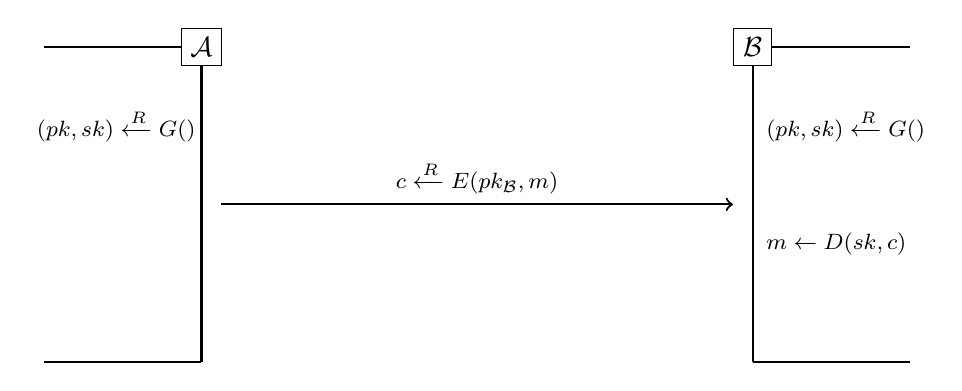
\begin{tikzpicture}
      \pause
        \node[draw] (AdversaryA) at (-3, 2) {\(\mathcal{A}\)}; 
        \draw[thick] (AdversaryA) -- ++(0, -4); 
        \draw[thick] (AdversaryA) -- ++(-2, 0);
        \draw[thick] (-3, -2) -- ++(-2, 0);
      \pause
        \node[draw] (ChallengerA) at (4,2) {\(\mathcal{B}\)}; 
        \draw[thick] (ChallengerA) -- ++(0, -4);
        \draw[thick] (ChallengerA) -- ++(2, 0);
        \draw[thick] (4, -2) -- ++(2, 0);

      \pause
        \node[draw=none,fill=none,anchor=east, font=\footnotesize] (choice0) at ($(AdversaryA) + (.05,-1)$) {\((pk, sk) \xleftarrow[]{R} G() \)};
        \node[draw=none,fill=none,anchor=west, font=\footnotesize] (choice0) at ($(ChallengerA) + (.05,-1)$) {\((pk, sk) \xleftarrow[]{R} G() \)};

      \pause
        \draw[->,thick] ($(AdversaryA)+(0.25,-2)$) -- ($(ChallengerA)+(-0.25,-2)$) node [pos=0.5,above,font=\footnotesize] {\(c \xleftarrow[]{R} E(pk_{\mathcal{B}}, m)\)};

      \pause
        \node[draw=none,fill=none,anchor=west, font=\footnotesize] (choice0) at ($(ChallengerA) + (.05,-2.5)$) {\(m \leftarrow D(sk, c)\)};

      \end{tikzpicture}
\end{frame}

\begin{frame}{Benefits}
    \begin{enumerate}
        \item \pause Public key encryption is often referred to as \textit{assymetric encryption} because the encryptor and decryptor use different keys (unlike \textit{symmetric encryption} which uses the same keys)
        \item \pause After the public key is securely obtained, there is only one interaction to send a message!
        \item \pause We can re-use the public key many times
        \item \pause Anyone can post their public key for everyone else to see (no key exchange required), this means that the secret keys must not be derivable from public keys
    \end{enumerate}
\end{frame}

\section{Semantic Security}

\begin{frame}{Review of Semantic Security}
  \begin{itemize}
    \item \pause The intuition of semantic security is that the probability a computationally bounded adversary can learn anything about a message from its ciphertext is negligible
    \item \pause Semantic security guarantees that a message cannot be recovered from a ciphertext
  \end{itemize}
\end{frame}

\begin{frame}{Public Key Semantic Security Attack Game}
    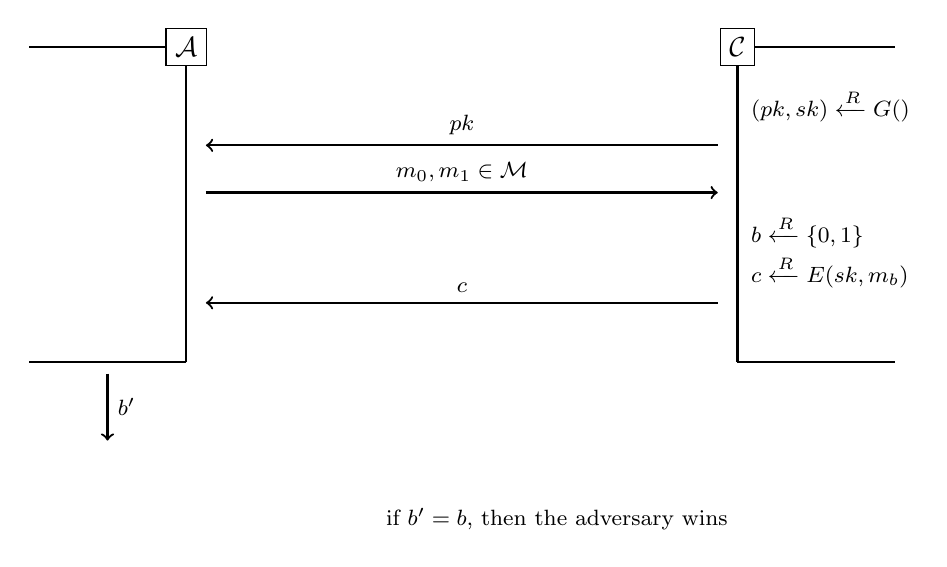
\begin{tikzpicture}
      \pause
        \node[draw] (AdversaryA) at (-3, 2) {\(\mathcal{A}\)}; 
        \draw[thick] (AdversaryA) -- ++(0, -4); 
        \draw[thick] (AdversaryA) -- ++(-2, 0);
        \draw[thick] (-3, -2) -- ++(-2, 0);
      \pause
        \node[draw] (ChallengerA) at (4,2) {\(\mathcal{C}\)}; 
        \draw[thick] (ChallengerA) -- ++(0, -4);
        \draw[thick] (ChallengerA) -- ++(2, 0);
        \draw[thick] (4, -2) -- ++(2, 0);

      \pause
        \node[draw=none,fill=none,anchor=west, font=\footnotesize] (choice0) at ($(ChallengerA) + (.05,-.75)$) {\((pk, sk) \xleftarrow[]{R} G() \)};

      \pause
        \draw[->,thick] ($(ChallengerA)+(-0.25,-1.25)$) -- ($(AdversaryA)+(0.25,-1.25)$) node [pos=0.5,above,font=\footnotesize] {\(pk\)};

      \pause
        \draw[->,thick] ($(AdversaryA)+(0.25,-1.85)$) -- ($(ChallengerA)+(-0.25,-1.85)$) node [pos=0.5,above,font=\footnotesize] {\(m_0, m_1 \in \mathcal{M}\)};

      \pause
        \node[draw=none,fill=none,anchor=west, font=\footnotesize] (choice0) at ($(ChallengerA) + (.05,-2.35)$) {\(b \xleftarrow[]{R} \{0, 1\}\)};
        \node[draw=none,fill=none,anchor=west, font=\footnotesize] (choice0) at ($(ChallengerA) + (.05,-2.85)$) {\(c \xleftarrow[]{R} E(sk, m_b)\)};

      \pause
        \draw[->,thick] ($(ChallengerA)+(-0.25,-3.25)$) -- ($(AdversaryA)+(0.25,-3.25)$) node [pos=0.5,above,font=\footnotesize] {\(c\)};

      \pause
        \draw[->,thick] ($(AdversaryA)+(-1,-4.15)$) -- ($(AdversaryA)+(-1, -5)$) node [pos=0.5,right,font=\footnotesize] {\(b'\)};

      \pause
        \node[draw=none,fill=none,anchor=east, font=\footnotesize] (choice0) at ($(ChallengerA) + (0, -6)$) {if \(b' = b\), then the adversary wins};

      \end{tikzpicture}
\end{frame}

\begin{frame}{Semantic Security Randomization}
  \begin{itemize}
    \item \pause For public key semantic security, the encryption function must be random. Can we think of an attack???
    \item \pause Future Homework Assignment!
  \end{itemize}
\end{frame}

\section{Chosen Plaintext Attack Security}

\begin{frame}{Public Key CPA Security}
  \begin{itemize}
    \item \pause Semantic security does not imply CPA security in symmetric key cryptography schemes
    \item \pause The intuition behind this is that in a symmetric key security setting, the attacker cannot encrypt their own messages into their own cipher texts (because they don't have access to the key)
    \item \pause In a public key setting, the adversary doesn't even need to interact with the challenger to get cipher texts
  \end{itemize}
\end{frame}

\begin{frame}{Public Key CPA Attack Game}
    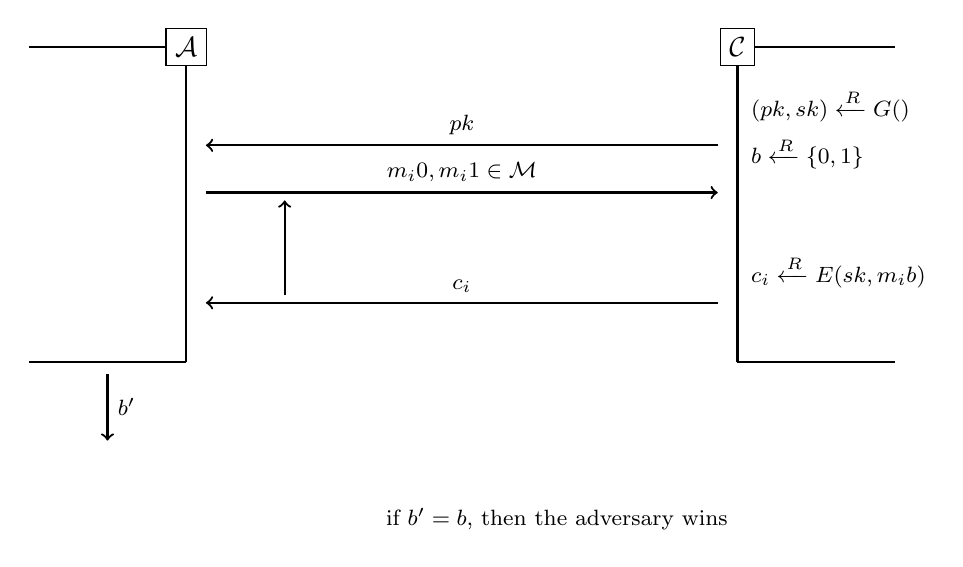
\begin{tikzpicture}
      \pause
        \node[draw] (AdversaryA) at (-3, 2) {\(\mathcal{A}\)}; 
        \draw[thick] (AdversaryA) -- ++(0, -4); 
        \draw[thick] (AdversaryA) -- ++(-2, 0);
        \draw[thick] (-3, -2) -- ++(-2, 0);
      \pause
        \node[draw] (ChallengerA) at (4,2) {\(\mathcal{C}\)}; 
        \draw[thick] (ChallengerA) -- ++(0, -4);
        \draw[thick] (ChallengerA) -- ++(2, 0);
        \draw[thick] (4, -2) -- ++(2, 0);

      \pause
        \node[draw=none,fill=none,anchor=west, font=\footnotesize] (choice0) at ($(ChallengerA) + (.05,-.75)$) {\((pk, sk) \xleftarrow[]{R} G() \)};
        \node[draw=none,fill=none,anchor=west, font=\footnotesize] (choice0) at ($(ChallengerA) + (.05,-1.35)$) {\(b \xleftarrow[]{R} \{0, 1\}\)};

      \pause
        \draw[->,thick] ($(ChallengerA)+(-0.25,-1.25)$) -- ($(AdversaryA)+(0.25,-1.25)$) node [pos=0.5,above,font=\footnotesize] {\(pk\)};

      \pause
        \draw[->,thick] ($(AdversaryA)+(0.25,-1.85)$) -- ($(ChallengerA)+(-0.25,-1.85)$) node [pos=0.5,above,font=\footnotesize] {\(m_i0, m_i1 \in \mathcal{M}\)};

      \pause
        \node[draw=none,fill=none,anchor=west, font=\footnotesize] (choice0) at ($(ChallengerA) + (.05,-2.85)$) {\(c_i \xleftarrow[]{R} E(sk, m_ib)\)};

      \pause
        \draw[->,thick] ($(ChallengerA)+(-0.25,-3.25)$) -- ($(AdversaryA)+(0.25,-3.25)$) node [pos=0.5,above,font=\footnotesize] {\(c_i\)};
        \draw[->,thick] ($(AdversaryA)+(1.25,-3.15)$) -- ($(AdversaryA)+(1.25, -1.95)$) node [pos=0.5,right,font=\footnotesize] {};

      \pause
        \draw[->,thick] ($(AdversaryA)+(-1,-4.15)$) -- ($(AdversaryA)+(-1, -5)$) node [pos=0.5,right,font=\footnotesize] {\(b'\)};

      \pause
        \node[draw=none,fill=none,anchor=east, font=\footnotesize] (choice0) at ($(ChallengerA) + (0, -6)$) {if \(b' = b\), then the adversary wins};

      \end{tikzpicture}
\end{frame}

\section{Chosen Ciphertext Attack Security}

\begin{frame}{CCA Motivation}
  \begin{itemize}
    \item \pause Imagine I collected homework by email and required that y'all encrypt your homework with my public key \(pk\)
    \item \pause What if another student intercepted that stream of data and strategically flipped bits until the submission read as "from: student1" to "from: student2"
    \item \pause Therefore, we need our systems to be secure against adversaries generating valid cipher texts
  \end{itemize}
\end{frame}

\begin{frame}{CCA Construction}
  \pause
  \[E(pk, m) = [x \xleftarrow[]{R} \mathcal{X}, y \leftarrow F(pk, x), k \leftarrow H(x), c \xleftarrow[]{R} E_s(k, m)] \rightarrow (c, y)\]
  \pause
  \[D(pk, (y, c)) = [x \leftarrow I(sk, y), k \leftarrow H(x), m \leftarrow D_s(k,c) ]\rightarrow m\]
\end{frame}

\section{Shamir Secret Sharing}

\begin{frame}{Motivation}
  \begin{itemize}
    \item \pause suppose you have a secret that you want to share with your friends
    \item \pause but you only want your friends to unlock this secret if they are all together
    \item \pause wouldn't it be cool if there was a mathematical way to ensure they can only unlock the secret if they are all together?
  \end{itemize}
\end{frame}

\begin{frame}{Overview}
  \begin{itemize}
    \item \pause Enter polynomial interpolation
    \item \pause if you have two points, you can find a unique line that intersects them, if you have 3 points, you can identify a unique parabola and so on
    \item \pause you can encode your secret somewhere along a function, and then tell all of your friends a different point along the curve expressed by the function
    \item \pause if enough of your friends get together, they can figure out the exact curve and and find the secret!
  \end{itemize}
\end{frame}

\end{document}